\documentclass[12pt, a4paper]{book}

\usepackage[T1]{fontenc}
\usepackage[utf8]{inputenc}
\usepackage[charter, cal=cmcal]{mathdesign}
\usepackage[scaled=0.92]{helvet}
\usepackage{geometry}
\geometry{a4paper, top=30mm, bottom=30mm, inner=32mm, outer=25mm, marginparwidth=18mm}

\usepackage{amsmath, amsthm}
\usepackage[version=4]{mhchem}
\usepackage{graphicx}
\usepackage[dvipsnames,svgnames,table]{xcolor}
\usepackage{tikz}
\usetikzlibrary{arrows.meta, shapes.geometric, positioning,
                calc, backgrounds, decorations.pathmorphing, patterns}
\usepackage{pgfplots}
\pgfplotsset{compat=1.18}
\usepackage{tcolorbox}
\tcbuselibrary{skins, breakable, theorems}
\usepackage{titlesec}
\usepackage{fancyhdr}
\usepackage{enumitem}
\usepackage{booktabs}
\usepackage{array}
\usepackage{multicol}
\usepackage{caption}
\usepackage{parskip}
\usepackage{siunitx}
\usepackage{pifont}
\usepackage[colorlinks=true, linkcolor=BrickRed,
            urlcolor=NavyBlue, citecolor=ForestGreen]{hyperref}

% ── Colours (Journey 2) ───────────────────────────────────────────────────────
\definecolor{JourneyColor}{HTML}{4A235A}
\definecolor{ModuleColor}{HTML}{6C3483}
\definecolor{PuzzleColor}{HTML}{1A5276}
\definecolor{DiscoveryColor}{HTML}{B7950B}
\definecolor{WarningColor}{HTML}{C0392B}
\definecolor{ProblemColor}{HTML}{117A65}
\definecolor{ReflectColor}{HTML}{1D6A39}
\definecolor{HistoryColor}{HTML}{6E2F1A}
\definecolor{LightBg}{HTML}{F8F9FA}
\definecolor{ElectronBlue}{HTML}{1565C0}
\definecolor{NucleusRed}{HTML}{B71C1C}
\definecolor{CrisisRed}{HTML}{7B241C}

% ── Boxes ─────────────────────────────────────────────────────────────────────
\newtcolorbox{puzzlebox}[1][]{enhanced,breakable,
  colback=PuzzleColor!6,colframe=PuzzleColor,fonttitle=\bfseries\sffamily,
  title={The Puzzle},attach boxed title to top left={yshift=-2mm,xshift=6mm},
  boxed title style={colback=PuzzleColor},borderline west={3pt}{0pt}{PuzzleColor},#1}

\newtcolorbox{discoverybox}[1][]{enhanced,breakable,
  colback=DiscoveryColor!8,colframe=DiscoveryColor,fonttitle=\bfseries\sffamily,
  title={Discovery},attach boxed title to top left={yshift=-2mm,xshift=6mm},
  boxed title style={colback=DiscoveryColor},borderline west={3pt}{0pt}{DiscoveryColor},#1}

\newtcolorbox{problembox}[1][]{enhanced,breakable,
  colback=ProblemColor!5,colframe=ProblemColor,fonttitle=\bfseries\sffamily,
  title={Problems},attach boxed title to top left={yshift=-2mm,xshift=6mm},
  boxed title style={colback=ProblemColor},borderline west={3pt}{0pt}{ProblemColor},#1}

\newtcolorbox{deepbox}[1][]{enhanced,breakable,
  colback=JourneyColor!5,colframe=JourneyColor,fonttitle=\bfseries\sffamily,
  title={Deep Problems},attach boxed title to top left={yshift=-2mm,xshift=6mm},
  boxed title style={colback=JourneyColor},borderline west={4pt}{0pt}{JourneyColor},#1}

\newtcolorbox{historybox}[1][]{enhanced,breakable,
  colback=HistoryColor!7,colframe=HistoryColor!60,fonttitle=\bfseries\sffamily\small,
  title={Historical Note},attach boxed title to top left={yshift=-2mm,xshift=6mm},
  boxed title style={colback=HistoryColor!80},#1}

\newtcolorbox{reflectionbox}[1][]{enhanced,breakable,
  colback=ReflectColor!6,colframe=ReflectColor,fonttitle=\bfseries\sffamily,
  title={Reflection},attach boxed title to top left={yshift=-2mm,xshift=6mm},
  boxed title style={colback=ReflectColor},borderline west={3pt}{0pt}{ReflectColor},#1}

\newtcolorbox{crisisbox}[1][]{enhanced,breakable,
  colback=CrisisRed!6,colframe=CrisisRed,fonttitle=\bfseries\sffamily,
  title={The Classical Crisis},attach boxed title to top left={yshift=-2mm,xshift=6mm},
  boxed title style={colback=CrisisRed},borderline west={4pt}{0pt}{CrisisRed},#1}

\newtcolorbox{namedconcept}[2][]{enhanced,
  colback=ModuleColor!6,colframe=ModuleColor,fonttitle=\bfseries\sffamily\large,
  title={#2},attach boxed title to top left={yshift=-2mm,xshift=6mm},
  boxed title style={colback=ModuleColor},#1}

% ── Section formatting ────────────────────────────────────────────────────────
\titleformat{\chapter}[display]
  {\normalfont\sffamily\huge\bfseries\color{JourneyColor}}
  {\textcolor{JourneyColor!60}{\chaptertitlename\ \thechapter}}{10pt}{\Huge}
  [\vspace{2pt}\textcolor{JourneyColor}{\titlerule[1.5pt]}]

\titleformat{\section}
  {\normalfont\sffamily\Large\bfseries\color{ModuleColor}}
  {\thesection}{1em}{}[\textcolor{ModuleColor!40}{\titlerule[0.6pt]}]

\titleformat{\subsection}
  {\normalfont\sffamily\large\bfseries\color{JourneyColor!80}}{\thesubsection}{1em}{}

\titleformat{\subsubsection}
  {\normalfont\sffamily\normalsize\bfseries}{\thesubsubsection}{1em}{}

\pagestyle{fancy}
\fancyhf{}
\fancyhead[LE]{\small\sffamily\textcolor{JourneyColor}{\leftmark}}
\fancyhead[RO]{\small\sffamily\textcolor{ModuleColor}{\rightmark}}
\fancyfoot[C]{\small\thepage}
\renewcommand{\headrulewidth}{0.4pt}

\newcommand{\newterm}[1]{\textit{\textcolor{DiscoveryColor}{#1}}}
\newcommand{\important}[1]{\textcolor{ModuleColor}{\textbf{#1}}}

% ══════════════════════════════════════════════════════════════════════════════
\begin{document}
\setcounter{chapter}{1}
\chapter[Journey 2 --- Architecture of the Atom]
        {Journey Two\\[8pt]
         \textcolor{ModuleColor}{\large Architecture of the Atom}}
\setcounter{section}{2}

% ══════════════════════════════════════════════════════════════════════════════
\section{Module 2.3 --- The Disaster of Classical Physics: Why Atoms Shouldn't Exist}
\label{sec:mod2.3}

\subsection*{Motivation}

We have built a picture of the atom that seems satisfying:
a dense positive nucleus at the centre, electrons orbiting
around it like planets around the sun.
Rutherford's scattering formula fits the data perfectly.

But there is a catastrophic problem lurking in this picture,
one that Rutherford and his colleagues were fully aware of.

Classical electrodynamics --- the theory of Maxwell,
developed and tested throughout the nineteenth century ---
makes an unambiguous prediction:
\emph{any accelerating charged particle must radiate
electromagnetic energy}.
An electron in a circular orbit is continuously
changing direction, which means it is continuously
accelerating.
Therefore it must continuously radiate.

As it radiates, it loses energy.
As it loses energy, it falls to a lower orbit,
which is smaller and faster.
As it moves faster, it radiates more.

The whole process runs away.
Calculation shows the electron should spiral into
the nucleus in approximately $10^{-11}$ seconds.

\begin{center}
\begin{tcolorbox}[enhanced, colback=CrisisRed!7, colframe=CrisisRed,
  width=0.88\textwidth, arc=3pt]
\centering\sffamily\normalsize\bfseries
The classical prediction:\\[6pt]
\normalfont\sffamily\small
The Rutherford atom should collapse in $\sim 10^{-11}$ seconds.\\[4pt]
But hydrogen atoms have been stable for $\sim 10^{10}$ years.\\[4pt]
\large\bfseries\color{CrisisRed}
Classical physics is wrong about the atom.
\end{tcolorbox}
\end{center}

This module explores exactly why classical physics fails,
what experimental evidence forced a new picture,
and what that new picture demands.

% ─── Section: The Classical Radiation Problem ─────────────────────────────────
\subsection{Why an Orbiting Electron Must Radiate}

The connection between acceleration and radiation
is one of the deepest results of classical electrodynamics.
A stationary charge produces a static electric field.
A charge moving at \emph{constant} velocity produces
a static field that travels with it.
But a charge that \emph{accelerates} --- changes its velocity ---
disturbs the field in a way that propagates outward as
an electromagnetic wave.

For a charge $q$ with acceleration $a$,
the radiated power is given by the \newterm{Larmor formula}:
\[
  P = \frac{q^2 a^2}{6\pi\varepsilon_0 c^3}
\]

For an electron in a circular orbit of radius $r$
around a proton (hydrogen atom), the centripetal
acceleration is:
\[
  a = \frac{v^2}{r} = \frac{e^2}{4\pi\varepsilon_0 m_e r^2}
\]
(using the condition that the electrostatic force provides
the centripetal force: $\frac{e^2}{4\pi\varepsilon_0 r^2} = \frac{m_e v^2}{r}$).

Substituting into the Larmor formula gives a radiated power
that depends on the orbit radius.
As $r$ decreases, $P$ increases --- a runaway process.

\begin{center}
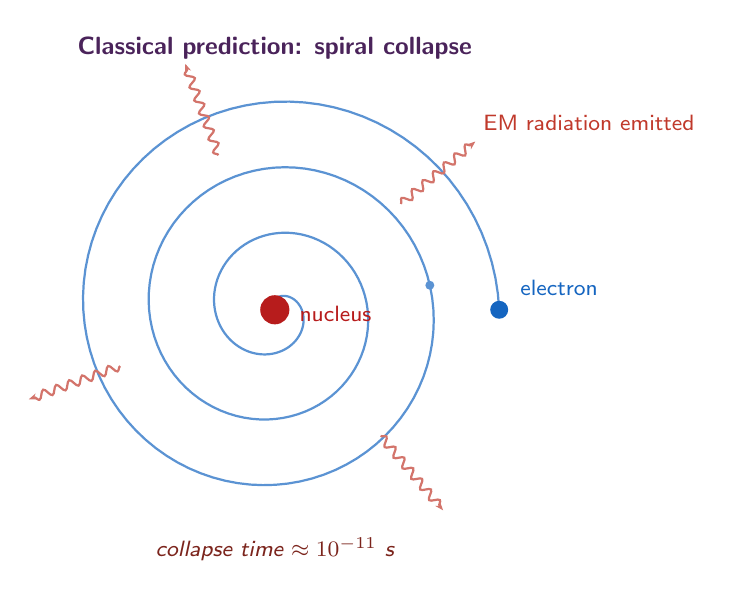
\begin{tikzpicture}[
  every node/.style={font=\sffamily\small},
  scale=0.95
]
  % Spiral orbit
  \node[font=\sffamily\small\bfseries, color=JourneyColor]
    at (0, 3.5) {Classical prediction: spiral collapse};

  % Draw a spiralling inward path (simple, no decoration markings)
  \draw[thick, ElectronBlue!70, domain=0:6.8*3.14159, samples=300,
    variable=\t]
    plot ({(3.0-\t*0.14)*cos(\t r)}, {(3.0-\t*0.14)*sin(\t r)});
  % Manual arrowheads at specific points along spiral
  \fill[ElectronBlue!70] ({(3.0-2.05*3.14159*0.14)*cos(2.05*3.14159 r)},
    {(3.0-2.05*3.14159*0.14)*sin(2.05*3.14159 r)}) circle (0.06cm);

  % Nucleus at centre
  \fill[NucleusRed] (0,0) circle (0.18cm);
  \draw[NucleusRed, thick] (0,0) circle (0.18cm);
  \node[font=\sffamily\footnotesize, text=NucleusRed, right]
    at (0.2,-0.05) {nucleus};

  % Radiation wavy arrows
  \foreach \angle in {40, 110, 200, 310}{
    \draw[-{Stealth[length=3pt]}, WarningColor!70, thick,
      decorate, decoration={snake, amplitude=1.5pt, segment length=5pt}]
      ({2.2*cos(\angle)},{2.2*sin(\angle)}) --
      ({3.5*cos(\angle)},{3.5*sin(\angle)});
  }
  \node[font=\sffamily\footnotesize, text=WarningColor]
    at (4.2, 2.5) {EM radiation emitted};

  % Time annotation
  \node[font=\sffamily\footnotesize\itshape, text=CrisisRed]
    at (0,-3.2) {collapse time $\approx 10^{-11}$ s};

  % Electron start
  \fill[ElectronBlue] ({3.0*cos(0 r)},{3.0*sin(0 r)}) circle (0.12cm);
  \node[font=\sffamily\footnotesize, text=ElectronBlue]
    at (3.8, 0.3) {electron};
\end{tikzpicture}
\end{center}

\begin{puzzlebox}
Before calculating the collapse time, think about what
the energy landscape looks like.

\begin{enumerate}[label=(\alph*), leftmargin=*]
  \item For a circular orbit, the total mechanical energy
        (kinetic + potential) is:
        \[
          E = -\frac{e^2}{8\pi\varepsilon_0 r}
        \]
        (This is derived from $F = ma$ for circular motion.)

        As $r$ \emph{decreases} (electron falls inward),
        does the total energy increase or decrease?
        Is the energy negative or positive, and what does
        the sign mean physically?

  \item The radiated power (energy lost per second) is:
        \[
          P = \frac{e^6}{12\pi\varepsilon_0^3 c^3 m_e^2 r^4}
        \]
        How does the power depend on orbit radius $r$?
        As the electron spirals inward (smaller $r$),
        what happens to the rate of radiation?
        Is this a stable or runaway process?

  \item The orbit \emph{frequency} (revolutions per second)
        for a circular orbit is:
        \[
          f = \frac{1}{2\pi}\sqrt{\frac{e^2}{4\pi\varepsilon_0 m_e r^3}}
        \]
        As $r$ decreases, what happens to the frequency?
        What frequency of electromagnetic radiation would
        you expect the electron to emit at each radius?

  \item From your answers to (b) and (c):
        as the electron spirals inward, the frequency of
        emitted radiation should continuously \emph{increase}.
        This predicts a \emph{continuous spectrum} ---
        a smooth sweep of frequencies.

        But when you heat hydrogen gas and look at the
        emitted light through a prism, you see sharp
        coloured lines at specific frequencies,
        not a continuous sweep.
        What does this tell you about the classical model?
\end{enumerate}
\end{puzzlebox}

% ─── Section: The Blackbody Problem ────────────────────────────────────────────
\subsection{The Blackbody Catastrophe: A Second Classical Failure}

The orbital instability of atoms was not the only way
classical physics failed at the atomic scale.
A second, completely independent failure involved
the radiation from hot objects.

Any object at temperature $T$ emits electromagnetic radiation.
The distribution of this radiation across frequencies
was measurable by 1900 with high precision.
Classical physics made a clear prediction for this distribution,
known as the \newterm{Rayleigh--Jeans law}:

\[
  u(\nu, T) = \frac{8\pi\nu^2}{c^3} k_B T
\]

where $u(\nu, T)$ is the energy per unit volume per unit
frequency, $\nu$ is frequency, and $k_B$ is Boltzmann's constant.

\begin{center}
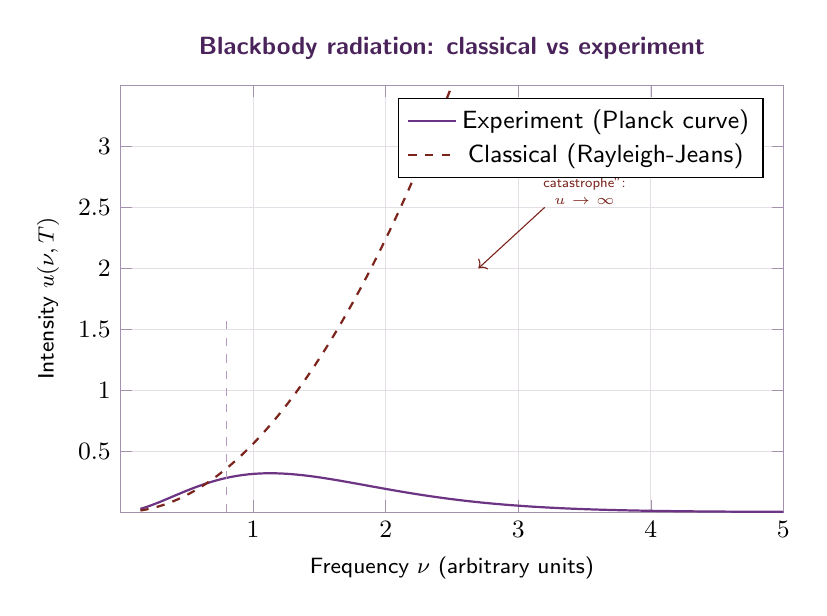
\begin{tikzpicture}[every node/.style={font=\sffamily\small}]
  \begin{axis}[
    width=10cm, height=7cm,
    xlabel={Frequency $\nu$ (arbitrary units)},
    ylabel={Intensity $u(\nu,T)$},
    xmin=0, xmax=5, ymin=0, ymax=3.5,
    xtick={1,2,3,4,5}, ytick={0.5,1.0,1.5,2.0,2.5,3.0},
    grid=both,
    grid style={line width=0.3pt, draw=JourneyColor!15},
    axis line style={color=JourneyColor!50},
    tick style={color=JourneyColor!50},
    title style={font=\sffamily\small\bfseries, color=JourneyColor},
    title={Blackbody radiation: classical vs experiment},
    label style={font=\sffamily\footnotesize},
    legend style={font=\sffamily\footnotesize, at={(0.97,0.97)},
                  anchor=north east},
    clip=true
  ]
    % Experimental (Planck) curve - peaks then falls
    \addplot[thick, color=ModuleColor, domain=0.15:5, samples=120]
      {3.5*(x^3)/(exp(2.5*x)-1)};
    \addlegendentry{Experiment (Planck curve)}

    % Classical Rayleigh-Jeans - goes to infinity
    \addplot[thick, dashed, color=CrisisRed, domain=0.15:2.8, samples=60]
      {0.56*x^2};
    \addlegendentry{Classical (Rayleigh-Jeans)}

    % Annotate the ultraviolet catastrophe
    \node[font=\sffamily\tiny, text=CrisisRed, align=center]
      at (axis cs:3.5, 2.7) {``ultraviolet\\catastrophe'':\\$u \to \infty$};
    \draw[->, thin, CrisisRed]
      (axis cs:3.2, 2.5) -- (axis cs:2.7, 2.0);

    % Peak of experimental
    \draw[dashed, thin, ModuleColor!50]
      (axis cs:0.8,0) -- (axis cs:0.8, 1.62);
    \node[font=\sffamily\tiny, text=ModuleColor]
      at (axis cs:0.8,-0.25) {$\nu_\text{max}$};
  \end{axis}
\end{tikzpicture}
\end{center}

\vspace{0.4em}

The classical prediction increases without limit at high
frequencies.
Integrating over all frequencies gives an \emph{infinite}
total energy for any object at any temperature.
This was called the \newterm{ultraviolet catastrophe}.

Every object at every temperature would radiate infinite
energy in infinite time.
Obviously this does not happen.
But classical physics had no way to stop it.

% ─── Section: Planck's Desperate Fix ─────────────────────────────────────────
\subsection{Planck's Desperate Hypothesis: Energy Comes in Packets}

In 1900, Max Planck found a mathematical formula that perfectly
described the observed blackbody spectrum.
To derive it, he needed to make an assumption so radical
he spent years trying to explain it away.

\begin{namedconcept}{Planck's Quantum Hypothesis (1900)}
The energy of electromagnetic oscillators at frequency $\nu$
is not continuous, but comes in discrete multiples of
a fundamental unit:
\[
  E = n h\nu \qquad n = 0, 1, 2, 3, \ldots
\]
where $h$ is \newterm{Planck's constant}:
\[
  h = 6.626 \times 10^{-34}\ \si{\joule\second}
\]
Energy is \newterm{quantised}: it cannot take arbitrary values,
only integer multiples of $h\nu$.
\end{namedconcept}

\vspace{0.5em}

With this assumption, the Planck distribution becomes:
\[
  u(\nu, T) = \frac{8\pi h \nu^3}{c^3} \cdot
              \frac{1}{e^{h\nu/k_BT} - 1}
\]

At low frequencies ($h\nu \ll k_BT$):
this reduces to the Rayleigh-Jeans law (classical behaviour).
At high frequencies ($h\nu \gg k_BT$):
the exponential in the denominator suppresses the radiation,
preventing the ultraviolet catastrophe.

\begin{historybox}
\textbf{Planck's Own Words on the Quantum}

Planck did not believe he had discovered something physically real.
He thought the quantisation was a mathematical trick ---
a way of making the calculation work, with no physical meaning.
He wrote that it was ``an act of desperation'' and spent years
trying to recover a classical derivation.

He never fully accepted the quantum.
When Einstein showed in 1905 that light itself comes in quanta
(not just the oscillators), Planck was among the sceptics.

The history of the quantum is filled with scientists who
made quantum discoveries and then spent years trying to
undo them.
Bohr, Einstein, Schr\"{o}dinger --- each contributed to quantum
theory and each had deep reservations about its implications.

This is unusual in science: normally, the person who
makes a discovery embraces it most enthusiastically.
The quantum was so strange that even its architects
struggled to accept it.
\end{historybox}

\begin{problembox}
\begin{enumerate}[label=\textbf{\arabic*.}]
  \item Calculate the energy of a single quantum (photon)
        of each of the following:
        \begin{enumerate}[label=(\alph*)]
          \item Red light, $\lambda = 700\ \si{\nano\metre}$
          \item Blue light, $\lambda = 450\ \si{\nano\metre}$
          \item X-ray, $\lambda = 0.1\ \si{\nano\metre}$
          \item Radio wave, $\lambda = 1\ \si{\metre}$
        \end{enumerate}
        Use $E = h\nu = hc/\lambda$,
        $h = 6.626\times10^{-34}\ \si{\joule\second}$,
        $c = 3.00\times10^8\ \si{\metre\per\second}$.

  \item The \newterm{Wien displacement law} says the peak
        frequency of blackbody radiation scales with temperature:
        \[
          \lambda_\text{max} T = 2.898\times10^{-3}\ \si{\metre\kelvin}
        \]
        \begin{enumerate}[label=(\alph*)]
          \item The surface of the sun is at $T \approx 5800\ \si{\kelvin}$.
                At what wavelength does it emit most strongly?
                What colour is this?
          \item A human body at $37\ \si{\celsius}$ --- at what
                wavelength does it emit most strongly?
                In what part of the spectrum is this?
          \item Night-vision cameras detect this radiation.
                Why can they see warm bodies in the dark?
        \end{enumerate}

  \item At room temperature ($T = 300\ \si{\kelvin}$),
        visible light has frequency
        $\nu \approx 6\times10^{14}\ \si{\hertz}$.
        \begin{enumerate}[label=(\alph*)]
          \item Calculate $h\nu$ for visible light.
          \item Calculate $k_B T$ (thermal energy per degree
                of freedom), where
                $k_B = 1.38\times10^{-23}\ \si{\joule\per\kelvin}$.
          \item Compare $h\nu$ and $k_BT$.
                If $h\nu \gg k_BT$, the Planck suppression
                factor $e^{h\nu/k_BT}$ is very large.
                Why does this explain why room-temperature
                objects do not glow with visible light?
        \end{enumerate}
\end{enumerate}
\end{problembox}

% ─── Section: Einstein's Photoelectric Effect ────────────────────────────────
\subsection{Einstein's Leap: Light Itself Is Quantised}

Planck's quantisation applied to oscillators.
In 1905, Einstein made a more radical claim:
\emph{light itself} consists of discrete packets of energy ---
quanta of light, which we now call \newterm{photons}.

His evidence came from the \newterm{photoelectric effect}.

\subsubsection{The Photoelectric Experiment}

When light shines on a metal surface, electrons are ejected.
This is the photoelectric effect.
Classical physics predicted:

\begin{itemize}[leftmargin=2em, nosep]
  \item Brighter light should give electrons more energy.
  \item Even dim light should eject electrons if you wait long enough.
  \item Any frequency of light should eject electrons.
\end{itemize}

The experiments showed something completely different:

\begin{center}
\begin{tabular}{p{5cm} p{4.5cm} p{4.5cm}}
\toprule
\textbf{Observation} & \textbf{Classical prediction} & \textbf{What really happens} \\
\midrule
Effect of brightness &
  More brightness $\to$ more energy per electron &
  More brightness $\to$ more electrons, same energy each \\[6pt]
Effect of frequency &
  Any frequency should work (given time) &
  Below threshold frequency $\nu_0$: NO electrons, ever \\[6pt]
Time delay &
  Dim light: wait and electrons appear &
  No delay: electrons appear instantly or not at all \\
\bottomrule
\end{tabular}
\end{center}

\vspace{0.5em}

Einstein's explanation: light comes in packets (photons),
each with energy $E = h\nu$.
A single photon must have enough energy to eject one electron.
The minimum energy needed to escape the metal is
the \newterm{work function} $\phi$.

\begin{namedconcept}{Einstein's Photoelectric Equation (1905)}
\[
  h\nu = \phi + \tfrac{1}{2}m_e v_\text{max}^2
\]
\vspace{-6pt}
\begin{itemize}[nosep, leftmargin=2em]
  \item $h\nu$ = energy of incoming photon
  \item $\phi$ = minimum energy to escape the metal (work function)
  \item $\tfrac{1}{2}m_e v_\text{max}^2$ = maximum kinetic energy
        of ejected electron
  \item Threshold frequency: $\nu_0 = \phi/h$
        (below this, $h\nu < \phi$ and no electron can escape)
\end{itemize}
\end{namedconcept}

\begin{center}
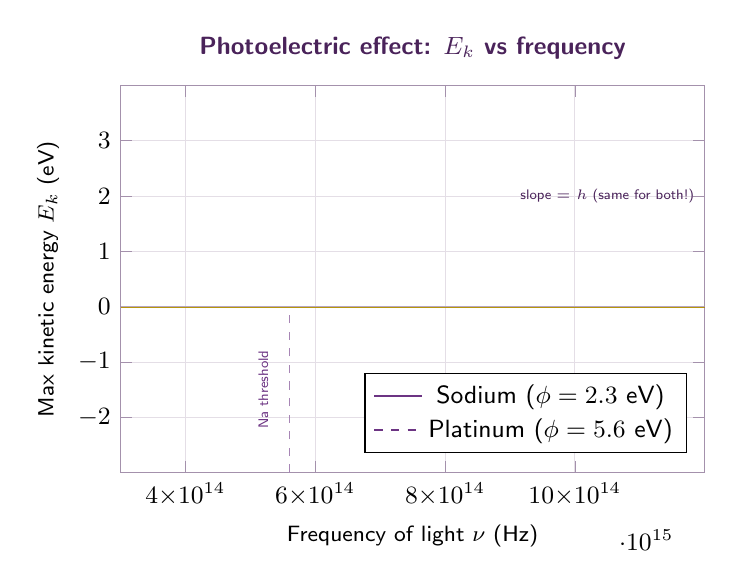
\begin{tikzpicture}[every node/.style={font=\sffamily\small}]
  \begin{axis}[
    width=9cm, height=6.5cm,
    xlabel={Frequency of light $\nu$ (Hz)},
    ylabel={Max kinetic energy $E_k$ (eV)},
    xmin=3e14, xmax=12e14,
    ymin=-3, ymax=4,
    xtick={4e14,6e14,8e14,10e14},
    xticklabels={$4{\times}10^{14}$,$6{\times}10^{14}$,
                 $8{\times}10^{14}$,$10{\times}10^{14}$},
    ytick={-2,-1,0,1,2,3},
    grid=both,
    grid style={line width=0.3pt, draw=JourneyColor!15},
    axis line style={color=JourneyColor!50},
    tick style={color=JourneyColor!50},
    title style={font=\sffamily\small\bfseries, color=JourneyColor},
    title={Photoelectric effect: $E_k$ vs frequency},
    label style={font=\sffamily\footnotesize},
    legend style={font=\sffamily\tiny, at={(0.97,0.05)},
                  anchor=south east}
  ]
    % Two metals with different work functions
    % Sodium: phi ~ 2.3 eV, threshold ~ 5.6e14 Hz
    \addplot[thick, color=ModuleColor, domain=5.6e14:12e14, samples=60]
      {4.136e-15*(x - 5.6e14)/1e14};
    \addplot[thick, dashed, color=ModuleColor,
             domain=3e14:5.6e14, samples=30]
      {0};
    \addlegendentry{Sodium ($\phi=2.3$ eV)}

    % Platinum: phi ~ 5.6 eV, threshold ~ 13.5e14 Hz
    \addplot[thick, color=DiscoveryColor, domain=3e14:12e14, samples=60]
      {4.136e-15*(x - 13.5e14)/1e14};
    \addlegendentry{Platinum ($\phi=5.6$ eV)}

    % Zero line
    \draw[thin, JourneyColor!40] (axis cs:3e14,0) -- (axis cs:12e14,0);

    % Threshold labels
    \draw[dashed, thin, ModuleColor!60]
      (axis cs:5.6e14,-3) -- (axis cs:5.6e14,0);
    \node[font=\sffamily\tiny, text=ModuleColor, rotate=90]
      at (axis cs:5.2e14,-1.5) {Na threshold};

    % Slope annotation
    \node[font=\sffamily\tiny, text=JourneyColor]
      at (axis cs:10.5e14, 2.0) {slope $= h$ (same for both!)};
  \end{axis}
\end{tikzpicture}
\end{center}

\vspace{0.4em}

The key experimental signature: the slope of $E_k$ vs $\nu$
is the same for all metals --- it equals $h$, Planck's constant.
Different metals have different intercepts (different work functions)
but the same slope.

This is compelling evidence for photons:
each photon transfers exactly $h\nu$ of energy,
regardless of which metal it hits.

\begin{problembox}
\begin{enumerate}[label=\textbf{\arabic*.}]
  \item Light of wavelength $\lambda = 250\ \si{\nano\metre}$
        strikes a sodium surface ($\phi = 2.3\ \si{\electronvolt}$).
        \begin{enumerate}[label=(\alph*)]
          \item Calculate the energy of one photon in eV.
                ($\SI{1}{eV} = 1.602\times10^{-19}\ \si{\joule}$;
                 $hc = 1240\ \si{eV\cdot nm}$)
          \item Does this photon have enough energy to eject
                an electron?
          \item Calculate the maximum kinetic energy of the
                ejected electron.
          \item Calculate the maximum speed of the ejected electron.
                ($m_e = 9.11\times10^{-31}\ \si{kg}$)
        \end{enumerate}

  \item The work function of zinc is
        $\phi = 4.3\ \si{\electronvolt}$.
        \begin{enumerate}[label=(\alph*)]
          \item What is the threshold frequency for zinc?
          \item What is the threshold wavelength?
          \item Red light ($\lambda = 700\ \si{nm}$) shines
                on zinc. Does anything happen?
          \item A student doubles the intensity of the red light.
                Does anything happen now?
                Explain using the photon model.
        \end{enumerate}

  \item Millikan measured the stopping voltage $V_s$ needed
        to halt photoelectrons (so that $eV_s = E_k$).
        His data for sodium:
        \begin{center}
        \begin{tabular}{cc}
        \toprule
        Frequency $\nu$ ($10^{14}$ Hz) & Stopping voltage $V_s$ (V) \\
        \midrule
        5.5 & 0.0 \\
        7.0 & 0.61 \\
        8.0 & 1.02 \\
        9.5 & 1.63 \\
        11.2 & 2.29 \\
        \bottomrule
        \end{tabular}
        \end{center}
        \begin{enumerate}[label=(\alph*)]
          \item Plot $eV_s$ (in eV) vs $\nu$.
          \item Find the slope. Compare to $h$.
          \item Find the threshold frequency and hence
                the work function of sodium.
        \end{enumerate}
\end{enumerate}
\end{problembox}

% ─── Section: Two Crises, One Resolution ──────────────────────────────────────
\subsection{Two Crises, One Resolution: The Quantum}

Let us step back and count the failures of classical physics
at the atomic scale by 1905.

\begin{center}
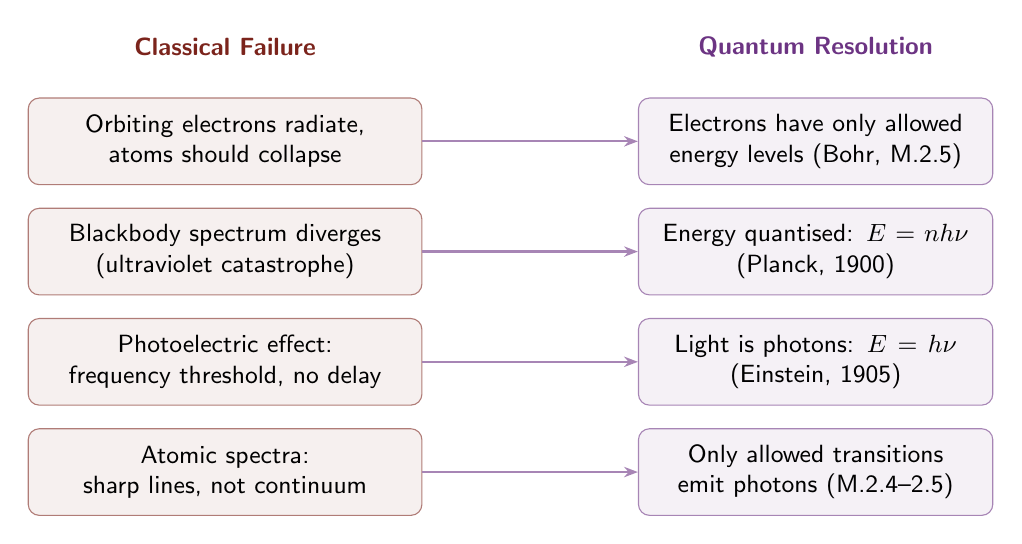
\begin{tikzpicture}[
  every node/.style={font=\sffamily\small, align=center},
  failbox/.style={draw=CrisisRed!60, fill=CrisisRed!7,
    rounded corners=4pt, minimum width=5cm, minimum height=1.1cm,
    text width=4.7cm},
  fixbox/.style={draw=ModuleColor!60, fill=ModuleColor!7,
    rounded corners=4pt, minimum width=4.5cm, minimum height=1.1cm,
    text width=4.2cm},
  arr/.style={-{Stealth[length=5pt]}, thick, color=ModuleColor!60}
]
  \node[font=\sffamily\small\bfseries, color=CrisisRed]
    at (-3.5, 4.0) {Classical Failure};
  \node[font=\sffamily\small\bfseries, color=ModuleColor]
    at (4.0, 4.0) {Quantum Resolution};

  \node[failbox] (f1) at (-3.5, 2.8)
    {Orbiting electrons radiate,\\atoms should collapse};
  \node[failbox] (f2) at (-3.5, 1.4)
    {Blackbody spectrum diverges\\(ultraviolet catastrophe)};
  \node[failbox] (f3) at (-3.5, 0.0)
    {Photoelectric effect:\\frequency threshold, no delay};
  \node[failbox] (f4) at (-3.5,-1.4)
    {Atomic spectra:\\sharp lines, not continuum};

  \node[fixbox] (q1) at (4.0, 2.8)
    {Electrons have only allowed\\energy levels (Bohr, M.2.5)};
  \node[fixbox] (q2) at (4.0, 1.4)
    {Energy quantised: $E=nh\nu$\\(Planck, 1900)};
  \node[fixbox] (q3) at (4.0, 0.0)
    {Light is photons: $E=h\nu$\\(Einstein, 1905)};
  \node[fixbox] (q4) at (4.0,-1.4)
    {Only allowed transitions\\emit photons (M.2.4--2.5)};

  \foreach \i in {1,2,3,4}
    \draw[arr] (f\i.east) -- (q\i.west);
\end{tikzpicture}
\end{center}

\vspace{0.5em}

The pattern is clear: in every case, the problem arises
because classical physics treats energy as continuous.
The quantum hypothesis --- energy comes in discrete packets ---
resolves all four failures simultaneously.

This is a profound convergence.
Four independent experimental anomalies all point to
the same conclusion from different directions.
Just as the five laws of Journey~1 all demanded atoms,
these four crises all demand quantisation.

\begin{crisisbox}
\textbf{The core conflict:}

Classical physics is built on the assumption that energy,
frequency, and all physical quantities vary continuously.
You can always have a little more or a little less.

Quantum mechanics is built on the discovery that at the atomic
scale, energy \emph{cannot} vary continuously.
It comes in minimum-sized packets, set by $h\nu$.

The size of the packet ($h\nu$) is so small
at human scales that the discreteness is invisible.
At atomic scales it dominates everything.

This is not a small correction to classical physics.
It is a completely different conception of physical reality.
\end{crisisbox}

% ─── Section: Deep Problems ───────────────────────────────────────────────────
\subsection*{Deep Problems}

\begin{deepbox}
\begin{enumerate}[label=\textbf{D\arabic*.}]

  \item \textbf{The Classical Collapse Time.}

        For the hydrogen atom, the energy of the electron
        in orbit at radius $r$ is:
        \[
          E(r) = -\frac{e^2}{8\pi\varepsilon_0 r}
        \]
        The power radiated (Larmor formula, simplified) is:
        \[
          P = \frac{e^6}{12\pi\varepsilon_0^3 m_e^2 c^3 r^4}
        \]
        Since $P = -dE/dt$ (energy is leaving), and using
        $dE/dr = \frac{e^2}{8\pi\varepsilon_0 r^2}$,
        we get $dr/dt = -P/(dE/dr)$.

        \begin{enumerate}[label=(\alph*)]
          \item Write $dr/dt$ in terms of $r$ and constants.
          \item Separate variables and integrate from
                $r = r_0 = 5.3\times10^{-11}$ m (Bohr radius)
                to $r = 0$.
          \item Calculate the collapse time numerically.
                Use SI values:
                $e = 1.602\times10^{-19}$ C,
                $\varepsilon_0 = 8.854\times10^{-12}$ C$^2$/Nm$^2$,
                $m_e = 9.11\times10^{-31}$ kg,
                $c = 3\times10^8$ m/s.
          \item Compare your answer to the age of the universe
                ($4\times10^{17}$ s). By how many orders of
                magnitude does the classical prediction fail?
        \end{enumerate}

  \item \textbf{The Energy of Quantisation.}

        At what scale does quantum behaviour become important?
        The criterion is roughly $h\nu \sim k_BT$
        (quantum energy $\sim$ thermal energy).

        \begin{enumerate}[label=(\alph*)]
          \item At room temperature ($T = 300$ K),
                what frequency $\nu$ satisfies $h\nu = k_BT$?
          \item What wavelength is this? What type of radiation?
          \item For frequencies \emph{below} this, is
                quantum behaviour significant or negligible
                at room temperature?
          \item A pendulum oscillates at 1 Hz.
                Calculate $h\nu_\text{pendulum}$ and $k_BT$
                at room temperature.
                By what factor does $k_BT$ exceed $h\nu$?
                Is quantum behaviour relevant for a pendulum?
          \item An electron in an atom oscillates at
                $\sim 10^{15}$ Hz.
                Repeat for this case.
                Is quantum behaviour relevant?
        \end{enumerate}

  \item \textbf{The Compton Effect: Photons Have Momentum.}

        Einstein's photon has energy $E = h\nu$.
        Since photons travel at the speed of light, special
        relativity requires their momentum to be $p = E/c = h\nu/c = h/\lambda$.

        In 1923, Arthur Compton scattered X-rays off electrons
        and found the scattered X-ray had a \emph{longer
        wavelength} than the incident X-ray.
        This is called the Compton effect.

        \begin{enumerate}[label=(\alph*)]
          \item If a photon loses energy in the collision,
                what happens to its frequency?
                To its wavelength?
          \item Compton derived the wavelength shift:
                \[
                  \Delta\lambda = \frac{h}{m_e c}(1-\cos\theta)
                \]
                where $\theta$ is the scattering angle.
                Calculate the maximum wavelength shift
                (at $\theta = 180°$, i.e., backward scatter).
          \item The quantity $h/(m_e c)$ is called the
                \newterm{Compton wavelength} of the electron.
                Calculate its numerical value.
          \item Why does the Compton effect definitively prove
                that photons carry momentum?
                Could a classical wave explain this result?
        \end{enumerate}

\end{enumerate}
\end{deepbox}

% ─── Reflection ───────────────────────────────────────────────────────────────
\subsection*{Reflection}

\begin{reflectionbox}
\begin{enumerate}[label=\textbf{R\arabic*.}]
  \item Classical physics worked extraordinarily well
        for two centuries --- it explained the motion of planets,
        the propagation of light, the flow of electricity.
        \textbf{What does it mean for a theory to ``fail''?}
        Is classical physics now useless, or does it remain
        valid under certain conditions?
        What determines which theory to use?

  \item Planck described his quantum hypothesis as ``an act
        of desperation.''
        Einstein proposed photons against the resistance
        of most physicists, including Planck.
        \textbf{What does this tell us about scientific progress?}
        Is it always driven by building systematically on
        prior knowledge, or can it require abandoning
        deeply held assumptions?

  \item The energy quantum $h\nu$ is extraordinarily small
        at human scales but dominates at atomic scales.
        \textbf{Why does nature have a ``scale'' below which
        the rules change?}
        Are there other examples from other sciences where
        rules that apply at one scale break down at another?

  \item We have now seen three ``impossible'' results:
        atoms are mostly empty space (Rutherford),
        energy is quantised (Planck), and light is made
        of particles (Einstein) --- yet light is also a wave
        (it diffracts and interferes).
        \textbf{How should we respond when experiments
        tell us something that seems logically contradictory?}
        Is there a way to hold two contradictory ideas
        simultaneously without abandoning reason?
\end{enumerate}
\end{reflectionbox}

\vspace{1.5em}
\begin{center}
\begin{tcolorbox}[enhanced, colback=DiscoveryColor!8, colframe=DiscoveryColor,
  width=0.88\textwidth, arc=3pt]
\centering\sffamily\small
\textbf{What we invented in this module.}\\[4pt]
We invented the photon and the energy quantum.
We did not do this by choice.
Classical physics, which worked magnificently at human scales,
gave catastrophically wrong answers for radiation from atoms.
The only cure was to accept that energy is discrete ---
that it comes in packets of size $h\nu$, where $h$ is
Planck's constant.
This is one of the two great revolutions of twentieth-century physics
(the other being relativity).
We still do not fully understand \emph{why} energy is quantised.
We only know that it is, and that every experiment confirms it.
\end{tcolorbox}
\end{center}

\vspace{2em}
\noindent\textcolor{JourneyColor!40}{\rule{\textwidth}{0.6pt}}
\begin{center}
\textit{\sffamily\small
Module 2.3 complete. Continue to Module 2.4:\\
\textbf{The Hydrogen Spectrum and the Birth of Quantisation}.}
\end{center}

\end{document}